\documentclass[12pt, a4paper, oneside]{ctexart}
\usepackage{amsmath, amsthm, amssymb, bm, color, graphicx, geometry, mathrsfs,extarrows, braket, booktabs, array, wrapfig}
\usepackage[colorlinks,linkcolor=red,anchorcolor=blue,citecolor=blue,urlcolor=blue,menucolor=black]{hyperref}
%%%% 设置中文字体 %%%%
\setCJKmainfont{方正新书宋_GBK.ttf}[BoldFont=方正小标宋_GBK, ItalicFont=方正楷体_GBK]
%%%% 设置英文字体 %%%%
\setmainfont{Times New Roman}
\setsansfont{Calibri}
\setmonofont{Consolas}

\linespread{1.4}
%\geometry{left=2.54cm,right=2.54cm,top=3.18cm,bottom=3.18cm}
\geometry{left=1.84cm,right=1.84cm,top=2.18cm,bottom=2.18cm}
\newcounter{problem}  % 问题序号计数器
\newenvironment{problem}[1][]{\stepcounter{problem}\par\noindent\textbf{题目\arabic{problem}. #1}}{\smallskip\par}
\newenvironment{solution}[1][]{\par\noindent\textbf{#1解答. }}{\smallskip\par}  % 可带一个参数表示题号\begin{solution}{题号}
\newenvironment{note}{\par\noindent\textbf{注记. }}{\smallskip\par}

%%%% 图片相对路径 %%%%
\graphicspath{{figure/}} % 当前目录下的figure文件夹, {../figure/}则是父目录的figure文件夹
\setlength{\abovecaptionskip}{-0.2cm}  % 缩紧图片标题与图片之间的距离
\setlength{\belowcaptionskip}{0pt} 

\everymath{\displaystyle} % 默认全部行间公式
\DeclareMathOperator*\uplim{\overline{lim}} % 定义上极限 \uplim_{}
\DeclareMathOperator*\lowlim{\underline{lim}} % 定义下极限 \lowlim_{}
\DeclareMathOperator*{\argmax}{arg\,max}  % 定义取最大值的参数 \argmax_{}
\DeclareMathOperator*{\argmin}{arg\,min}  % 定义取最小值的参数 \argmin_{}
\let\leq=\leqslant % 将全部leq变为leqslant
\let\geq=\geqslant % geq同理

%%%% 一些宏定义 %%%%
\def\bd{\boldsymbol}        % 加粗(向量) boldsymbol
\def\disp{\displaystyle}    % 使用行间公式 displaystyle(默认)
\def\tsty{\textstyle}       % 使用行内公式 textstyle
\def\sign{\text{sign}}      % sign function
\def\wtd{\widetilde}        % 宽波浪线 widetilde
\def\R{\mathbb{R}}          % Real number
\def\N{\mathbb{N}}          % Natural number
\def\Z{\mathbb{Z}}          % Integer number
\def\Q{\mathbb{Q}}          % Rational number
\def\C{\mathbb{C}}          % Complex number
\def\K{\mathbb{K}}          % Number Field
\def\P{\mathbb{P}}          % Polynomial
\def\N{\mathbb{N}}          % Natural number
\def\Z{\mathbb{Z}}          % Integer number
\def\E{\mathbb{E}}          % Exception
\def\var{\text{Var}}        % Variance
\def\bias{\text{bias}}      % bias
\def\d{\mathrm{d}}          % differential operator
\def\e{\mathrm{e}}          % Euler's number
\def\i{\mathrm{i}}          % imaginary number
\def\re{\mathrm{Re}}        % Real part
\def\im{\mathrm{Im}}        % Imaginary part
\def\res{\mathrm{Res}}      % Residue
\def\L{\mathcal{L}}         % Loss function
\def\wdh{\widehat}          % 宽帽子 widehat
\def\ol{\overline}          % 上横线 overline
\def\ul{\underline}         % 下横线 underline
\def\add{\vspace{1ex}}      % 增加行间距
\def\del{\vspace{-1.5ex}}   % 减少行间距

%%%% 定理类环境的定义 %%%%
\newtheorem{theorem}{定理}

%%%% 基本信息 %%%%
\newcommand{\RQ}{\today} % 日期
\newcommand{\km}{实变函数} % 科目
\newcommand{\bj}{强基数学002} % 班级
\newcommand{\xm}{吴天阳} % 姓名
\newcommand{\xh}{2204210460} % 学号

\begin{document}
\begin{center}
    \zihao{3}\textbf{数学建模大作业笔记}
\end{center}\vspace{-0.2cm}

% 正文部分
\subsection*{K均值}

设样本坐标集合为 $D = \{\bd{x}_1,\cdots,\bd{x}_n\}$,对应的权重为该建筑中人口数 $\{w_1,\cdots, w_n\}$,初始 $k$ 个质心位置随机从 $n$ 个点坐标中选取记为 $\{\bd{\mu}_1,\cdots,\bd{\mu}_k\}$.

\noindent\textbf{第一步}:计算每个样本点到最近的质心编号,对于样本点$\bd{x}_j$其所属的质心为
\begin{equation*}
    \lambda_j = \argmin_{1\leq i\leq k}||\bd{x}_j-\bd{\mu}_i||_2,
\end{equation*}
\textbf{第二步}:将其划分到该质心的集合中
\begin{equation*}
    C_{\lambda_j} \leftarrow C_{\lambda_j}\cup \{j\},
\end{equation*}
\textbf{第三步}:计算新质心向量
\begin{equation*}
    \bd{\mu}_i'= \frac{1}{\sum\limits_{j\in C_i}w_j}\sum_{j\in C_i}w_j\bd{x}_j.
\end{equation*}
若$\max_{1\leq i\leq k}||\bd{\mu}_i-\bd{\mu}_i'||_2 < 10^{-5}$则停止算法,否则更新$\mu_i\leftarrow \mu_i',\ (1\leq i\leq k)$,回到第一步继续迭代.

\subsection*{打分模型}

对于K均值得到的质心$\{\bd{\mu}_1,\cdots,\bd{\mu}_k\}$,如下进行评分
\begin{equation*}
    score = \frac{\disp\frac{2}{k(k-1)}\left(\sum_{1\leq i < j\leq k}||\bd{\mu}_i-\bd{\mu}_j||_2\right)}{\disp\sum_{1\leq i\leq k}\frac{1}{||C_i||}\sum_{j\in C_i}\frac{||\bd{x}_i-\bd{\mu}_i||_2}{w_j}}
\end{equation*}
分子表示质心两两之间的平均距离尽可能大;分母表示每个质心包含的样本距离应尽可能近,并且人口数量越多的所具有的权重更高,即对每个质心所包含的的样本距离进行加权平均,最后再对所有质心进行求和.

当$k=3$时,执行$2000$次K均值算法得到稳定的最优解,三个质心分别为:\\$(23,22), (44, 55), (67, 25)$(对坐标进行四舍五入).

当$k=6$时,执行$2000$次K均值算法得到稳定的最优解,六个质心分别为:\\$(13, 32), (37, 8), (38, 57), (63, 41), (64, 11), (75, 61)$(对坐标进行四舍五入).

\subsection*{压缩监测方案}
设混检比例为$k:1$,人群中感染新冠的概率为$p$,则一组中无阳性的概率为$(1-p)^k$,若存在至少一个阳性的概率为$1-(1-p)^k$,该组检测出阳性,则其中每个人进行单人单测. 设每人使用试剂盒个数为$X$,则
\begin{equation*}
    P(X = \frac{1}{k}) = (1-p)^k,\quad P(1+\frac{1}{k})=1-(1-p)^k,
\end{equation*}
于是$\E(X) = \frac{1}{k}(1-p)^k+\left(1+\frac{1}{k}\right)(1-(1-p)^k)=1+\frac{1}{k}-(1-p)^k$.\add

问题转化为给定$p$,求解$\E(X)$的最小值,可通过近似计算求解.

\textbf{基于人均成本的最优K值计算}:假设混合比例为$k:1$,总人数为$n$,由于每人采样费为$10$元,试剂盒价格为$30$元,则每人使用试剂盒的期望个数为$\E(X)=1+\frac{1}{k}-(1-p)^k$,每人期望采样次数为$1+(1-(1-p)^k)$,于是人均期望成本为
\begin{equation*}
    10(1+(1-(1-p)^k))+30(\frac{1}{k}+1-(1-p)^k) = 10+\frac{30}{k}+40(1-(1-p)^k)
\end{equation*}

\subsection*{第三问计算可转移采样点个数}
假设两个社区的人数分别为$N_1,N_2$,人均采样时间为$t$秒,采样点在两个社区移动所花时间为$T$分钟,采样至多所用时间$A$小时,则采样点应满足
\begin{equation*}
    \frac{t\cdot N_1}{k}+\frac{t\cdot N_2}{k}+T\times 60\leq A\times 3600
\end{equation*}
则
\begin{equation*}
    k\geq \frac{t\cdot(N_1+N_2)}{A\times 3600-T\times 60}
\end{equation*}
取$t = 28,\ A = 12,\ T = 20$最终结果向上取整,即
\begin{equation*}
    k=\left[\frac{28\times(N_1+N_2)}{12\times3600-20\times 60}\right]+1
\end{equation*}

% 下面给一些功能的写法
\iffalse
% 图片模板
\centerline{
    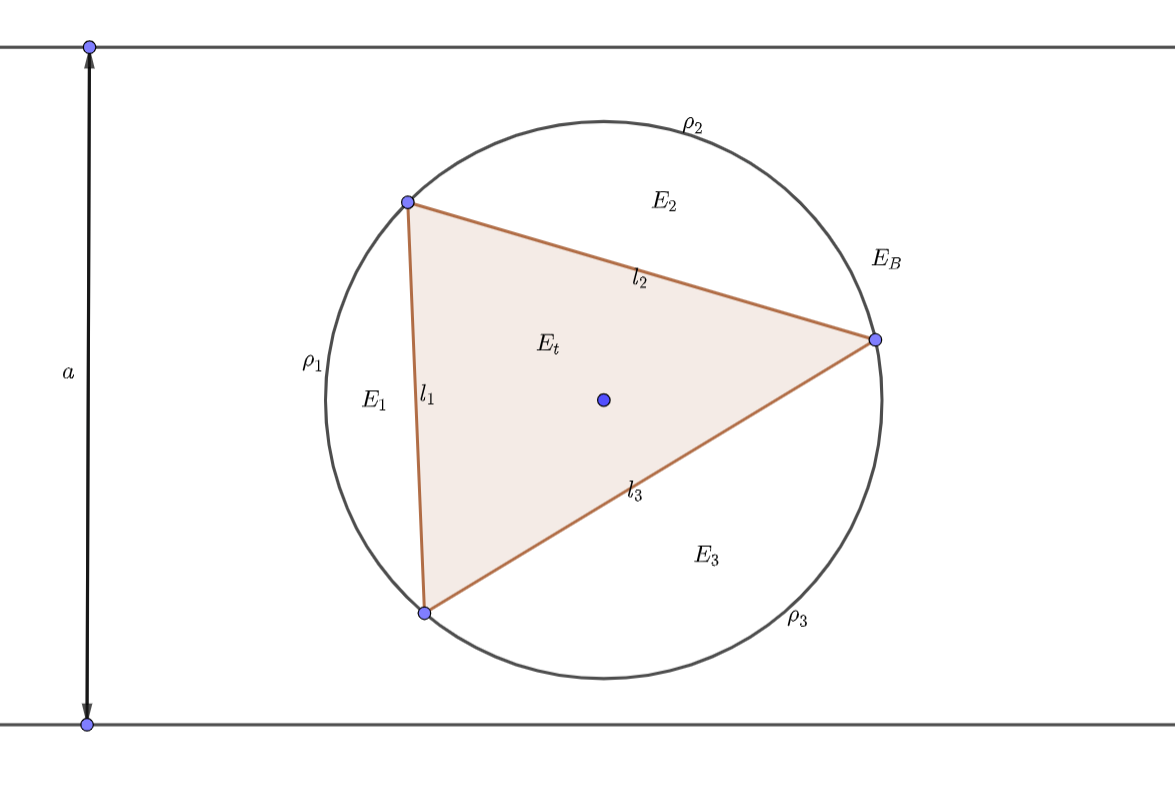
\includegraphics[width=0.8\textwidth]{figure.png}
}
% 表格模板
\renewcommand\arraystretch{0.8} % 设置表格高度为原来的0.8倍
\begin{table}[!htbp] % table标准
    \centering % 表格居中
    \begin{tabular}{p{1cm}<{\centering}p{1cm}<{\centering}p{3cm}<{\centering}p{5cm}<{\centering}} % 设置表格宽度
    %\begin{tabular}{cccc}
        \toprule
        $x_i$ & $f[x_1]$ & $f[x_i,x_{i+1}]$ & $f[x_i,x_{i+1},x_{i+2}]$ \\
        \midrule
        $x_0$ & $f(x_0)$ &                  &                          \\
        $x_0$ & $f(x_0)$ & $f'(x_0)$        &                          \\
        $x_0$ & $f(x_1)$ & $\frac{f(x_1)-f(x_0)}{x_1-x_0}$ & $\frac{f(x_1)-f(x_0)}{(x_1-x_0)^2}-\frac{f'(x_0)}{x_1-x_0}$\\
        \bottomrule
    \end{tabular}
\end{table}

\def\Log{\text{Log}} % 一个简单的宏定义
$\Log$ % 调用方法
\fi

\end{document}